\chapter{Perliminares}

\section{Estado de la cuestión}

\section{Pequeña introducción a la música}\label{sec:arm:armonia}

\label{arm:notas_musicales}
Sintetizando, nos centraremos en el estándar occidental, utilizado prácticamente en todas canciones que escuchamos diariamente, en el que los sonidos se dividen en conjuntos de 12 notas musicales, cada una con un nombre diferente, difiniendo nota musical como un símbolo que representa una frecuencia determinada. Para entender de dónde viene esta división utilizaremos como base la nota A4 (La4), con una frecuencia de 440Hz y duplicaremos su frecuencia a 880Hz, obteniendo así A5 (La5). Estas dos notas comparten nombre, ya que si las escucháramos nos sonarían muy familiares entre sí. Esto tiene una explicación física: al reproducir esa frecuencia (frotando una cuerda, elevando una columna de aire...), no solo se genera la frecuencia fundamental, sino que también se producen armónicos, que son múltiplos enteros de la frecuencia fundamental. 

Se llama octava a la distancia que separa una frecuencia de su duplicación, esto explica ahora los número escritos al lado de cada nota musical: A3 = 220Hz, A4 = 440Hz, A5 = 880Hz. Sabiendo esto se decidió entonces dividir la octava en 12 notas musicales, perceptualmente equidistantes, la cual difiere con una equidistancia a nivel de frecuencia, debido a la naturaleza exponencial de las frecuencias. Es la llamada afinación temperada. Sacamos como conclusión que el conjunto de sonidos utilizados está comprendido por las 12 notas musicales, cada una puediéndose encontrar en una octava distinta. 

Entrando en otra capa de profundidad, ese conjunto de notas musicales que conformar una canción puede ser dividida en dos partes:
\begin{enumerate}
    \item[\textbullet] \textbf{Melodía}: línea principal o motivo musical que guía la dirección y el desarrollo de una pieza musical. Es la parte más reconocible de una canción. En una composición musical es la que generalmente se canta o se toca de manera prominente.
    \item[\textbullet] \textbf{Armonía}: combinación simultánea de dos o más notas que se escuchan juntas y que suenan de manera agradable o consonante. La armonía proporciona un acompañamiento sonoro a la melodía principal y contribuye a enriquecer la textura musical. Se compone de acordes, que son grupos de notas tocadas simultáneamente.
\end{enumerate}

\section{Pequeña introducción a la armonía}

Como se acaba de explicar, la armonía se define como la combinación y disposición de notas musicales que suenan de manera agradable y coherente entre sí. Para entender tanto la armonía, como los algoritmos que se quieren mostrar en este apartado del TFG, es necesario interiorizar los siguientes conceptos, que se intentarán explicar de la manera más resumida posible. Cabe recalcar que la explicación se realiza en el contexto de la armonía moderna, la cual difiere en algunos puntos de la clásica, sin embargo, al tratarse de una introducción, la mayoría de conceptos que van a ser mostrados se comparten entre ambas doctrinas. A pesar de ello, una de las primeras cosas en las que sí difieren es en el nombre de las notas. A partir de ahora se utilizará cifrado americano: (\ref{tab:cifrado_americano})

\begin{table}[h]
    \centering
    \begin{tabular}{c||c|c|c|c|c|c|c}
        \textbf{Nota} & Do & Re & Mi & Fa & Sol & La & Si \\
        \hline
        \textbf{Cifrado} & C & D & E & F & G & A & B \\
    \end{tabular}
    \caption{Cifrado Americano}
    \label{tab:cifrado_americano}
\end{table}    

\subsection{Intervalos}\label{sec:arm:intervalos}

\begin{figure}[h]
    \centering
    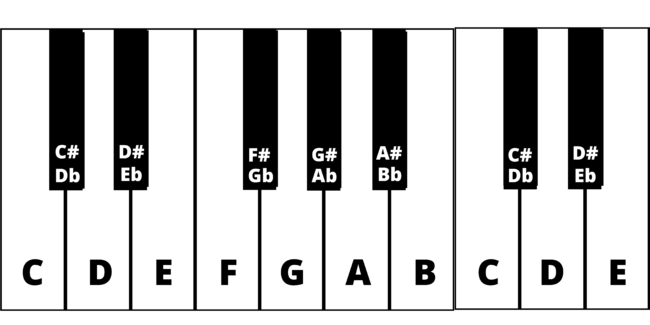
\includegraphics[width = 0.5\textwidth]{Imagenes/Bitmap/piano.png}
    \caption{Notas en el Piano}
    \label{fig:pianoImage}
\end{figure}

Un intervalo es la distancia que existe entre dos notas. Un semitono es la distancia mínima que puede existir entre dos notas. Un tono es igual a dos semitonos. Por ejemplo, enl piano \ref{fig:pianoImage} se puede comprobar fácilmente que la distancia entre el primer C y el primer E es de 4 semitonos (las teclas negras también cuentan como notas musicales aunque tengan nombres un poco especiales). Podemos encontrar esa distancia mínima de un semitono entre C y C\# o entre E y F, por ejemplo. Dependiendo del número de semitonos que tenga un intervalo, este tendrá un nombre y simbología diferente (\ref{tab:tabla_intervalos}). A estos intervalos también se les conoce como grados en ciertos contextos que veremos posteriormente. El número de semitonos que representan es el mismo, el único cambio es que el cardinal pasa a ser representado por un número romano.

\begin{table}[h]
    \centering
    \begin{tabular}{c|c|c}
        \textbf{Símbolo (grado)} & \textbf{Nombre} & \textbf{Nº Semitonos} \\
        \hline
        1 (T) & Tónica & 0 \\
        b2 & Segunda menor & 1 \\
        2 & Segunda Mayor & 2 \\
        b3 & Tercera menor & 3 \\
        3 & Tercera Mayor & 4 \\
        4 & Cuarta Justa & 5 \\
        \#4 & Cuarta Aumentada & 6 \\
        5b & Quinta disminuida & 6 \\
        5 & Quinta Justa & 7 \\
        b6 & Sexta menor & 8 \\
        6 & Sexta Mayor & 9 \\
        b7 & Séptima menor & 10 \\
        7 & Séptima Mayor & 11 \\
        8 & Octava & 12 \\
    \end{tabular}
    \caption{Tabla de Intervalos}
    \label{tab:tabla_intervalos}
\end{table}

Al observar la tabla (\ref{tab:tabla_intervalos}) se puede deducir por contexto que el símbolo 'b' (bemol) reduce en uno el número de semitonos del grado original, así como el símbolo '\#' (sostenido) los aumenta en uno. Por ejemplo, \#6 sería equivalente a una séptima menor (b7), con 10 semitonos ambos. Así mismo estos símbolos se pueden apilar, por ejemplo, bb7 sería equivalente a una sexta Mayor (6), con 9 semitonos ambos.

Con la información de esta tabla, ya podríamos entender afirmaciones tales como 'la quinta Justa de C es G' o 'la tercera Mayor de B es D\#', por ejemplo, si nos ponemos a contar los semitonos más detenidamente (piano de referencia en \ref{fig:pianoImage}).

Cabe recalcar que, evidentemente, existen intervalos que se salen de la octava, con más de 12 semitonos. Algunos no muy lejanos tienen incluso nombre propio, por ejemplo, una novena Mayor (9), de 14 semitonos. A pesar de ello, lo que se hará en estos casos es interpretar ese intervalo como su relativo si la nota estuviese en el 'mismo rango' que la tónica (nota desde la cual se mide el intervalo). Así, una novena Mayor sería equivalente a una segunda Mayor, de 2 semitonos y un intervalo de 42 semitonos será interpretado como una quinta disminuida (42 mod 12 = 6 semitonos), por ejemplo. De hecho, siguiendo esta definición, el propio intervalo de octava es redundante, ya que esta es equivalente a la tónica y cumple la misma función (12 mod 12 = 0 semitonos). Por ejemplo, la octava de C4 es C5. Por ello, el intervalo de octava también se debería quitar de la lista.

\subsection{Escalas}\label{sec:arm:escalas}

Se define escala como conjunto de 2 a 12 intervalos o grados ascencentes cuyo primer intervalo es siempre la tónica. Tradicionalmente, la mayoría de escalas están formadas por 7 grados, las más utilizadas en la música que escuchamos hoy en día son la Mayor y la menor (\ref{tab:escalas}).

\begin{table}[h]
    \centering
    \begin{tabular}{c|c|c|c|c|c|c|c}
        \textbf{Escala Mayor} & 1 (T) & 2 & 3 & 4 & 5 & 6 & 7 \\
        \hline
        \hline
        \textbf{Escala menor} & 1 (T) & 2 & b3 & 4 & 5 & b6 & b7 \\
    \end{tabular}
    \caption{Escalas Mayor y menor}
    \label{tab:escalas}
\end{table}

Este conjunto de intervalos representa una especie de esqueleto, un molde con el cual se puede crear una sucesión de notas musicales si se establece como tónica cualquiera de las 12 notas existentes. Aquí uno cuantos  ejemplos, utilizando como tónicas C, D y Bb: (\ref{tab:escalas_tonicas})

\begin{table}[h]
    \centering
    \begin{tabular}{c|c|c|c|c|c|c|c}
        \textbf{C Mayor} & C (T) & D & E & F & G & A & B \\
        \hline
        \textbf{D Mayor} & D (T) & E & F\# & G & A & B & C\# \\
        \hline
        \textbf{Bb Mayor} & Bb (T) & C & D & Eb & F & G & A \\
        \hline
        \hline
        \textbf{C menor} & C (T) & D & Eb & F & G & Ab & Bb \\
        \hline
        \textbf{D menor} & D (T) & E & F & G & A & Bb & C \\
        \hline
        \textbf{Bb menor} & Bb (T) & C & Db & Eb & F & Gb & Ab \\
    \end{tabular}
    \caption{Escalas y Tónicas}
    \label{tab:escalas_tonicas}
\end{table}

A parte de estas dos escalas, existen muchas otras más que se utilizan regularmente a la hora de componer música. Incluso existen compositores más vanguardistas que inventan nuevos conjuntos de grados, experimentando con nuevas formas de escribir música. Algunos ejemplos: (\ref{tab:otras_escalas})

\begin{table}[h]
    \centering
    \begin{tabular}{c|c|c|c|c|c|c|c}       
        \textbf{pentatónica Mayor} & 1 (T) & 2 & 3 & 5 & \multicolumn{1}{c}{6} \\
        \hline
        \textbf{pentatónica menor} & 1 (T) & b3 & 4 & 5 & \multicolumn{1}{c}{b6} \\
        \hline
        \textbf{hexatónica} & 1 (T) & 2 & 3 & \#4 & \#5 & \multicolumn{1}{c}{\#6}  \\
        \hline
        \textbf{frigia} & 1 (T) & b2 & b3 & 4 & 5 & b6 & b7 \\
        \hline
        \textbf{mixolidia} & 1 (T) & 2 & 3 & 4 & 5 & 6 & b7 \\
        \hline
        \textbf{menor armónica} & 1 (T) & 2 & b3 & 4 & 5 & b6 & 7 \\      
    \end{tabular}
    \caption{Otras Escalas}
    \label{tab:otras_escalas}
\end{table}

\subsection{Acordes}\label{sec:arm:acordes}

Aunque no todo el mundo estaría de acuerdo con esta definición, vamos a decir que un acorde es un conjunto de dos o más notas tocadas de forma simultánea. La definición es en cierta medida similar a la de una escala, ya que un acorde no deja de ser un conjunto de intervalos ascendentes, en el que el primero es simpre la tónica del acorde. También se cumple esa propiedad de 'molde' a la hora de establecer una nota musical como tónica del acorde. Los acordes más comunes están formados por tres notas (tríadas) y dependiendo del conjunto de intervalos se pueden conseguir diferentes sonoridades: (\ref{tab:triads} y \ref{tab:triadsC})

\begin{table}[h]
    \centering
    \begin{tabular}{c|c|c|c|c}       
        \textbf{Nombre} & \textbf{Símbolo} & \multicolumn{3}{c}{\textbf{Intervalos}} \\
        \hline
        \hline
        \textbf{Acorde Mayor} & & 1 (T) & 3 & 5 \\
        \hline
        \textbf{Acorde menor} & - & 1 (T) & b3 & 5 \\
        \hline
        \textbf{Acorde Aumentado} & + & 1 (T) & 3 & \#5 \\
        \hline
        \textbf{Acorde disminuido} & -b5 & 1 (T) & b3 & b5 \\
    \end{tabular}
    \caption{tríadas}
    \label{tab:triads}
\end{table}

\begin{table}[h]
    \centering
    \begin{tabular}{c|c|c|c|c}       
        \textbf{Nombre} & \textbf{Símbolo} & \multicolumn{3}{c}{\textbf{Notas}} \\
        \hline
        \hline
        \textbf{C Mayor} & C & C (T) & E & G \\
        \hline
        \textbf{C menor} & C- & C (T) & Eb & G \\
        \hline
        \textbf{C Aumentado} & C+ & C (T) & E & G\# \\
        \hline
        \textbf{C disminuido} & C-b5 & C (T) & Eb & Gb \\
    \end{tabular}
    \caption{tríadas en C}
    \label{tab:triadsC}
\end{table}

\label{arm:armonia_escala}
Se define como armonía de una escala el conjunto de acordes que se pueden formar utilizando únicamente las notas (o intervalos) de la escala. Esto puede chocar con la definición de acorde, ya que, como tal, puede haber miles de tipos de acordes diferentes si atendemos a toda la combinatoria, así que, por ahora, solo tendremos en cuenta los tipos de acordes definidos anteriormente, es decir, acordes mayores, menores, aumentados y disminuidos. Este concepto es más difícil de deducir y explicar, así que recomiendo la visualización de \href{https://www.youtube.com/watch?v=dMwVB3BWcjI}{este vídeo} en el que el autor encuentra la armonía de la escala C Mayor y pasa el resultado a grados, además de repasar otros conceptos vistos por encima anteriormente. Se obtiene el siguiente resultado: (\ref{tab:grados_C})

\begin{table}[h]
    \centering
    \begin{tabular}{c|c||c|c}
        \textbf{Grado} & \textbf{Acorde} & \textbf{Nota} & \textbf{Acorde} \\
        \hline
        I (T) &  & C (T) & C \\
        II & - & D & D- \\
        III & - & E & E- \\
        IV &  & F & F \\
        V &  & G & G \\
        VI & - & A & A- \\
        VII & -b5 & B & B-b5 \\
    \end{tabular}
    \caption{Escala Mayor en Grados y en C}
    \label{tab:grados_C}
\end{table}

Como se puede observar, en la escala Mayor se forma una tríada mayor a partir de los grados 1, 4 y 5, una menor a partir de los grados 2, 3 y 6, una disminuida a partir del grado 7 y no existe ningún grado del cual se forme una tríada aumentada. Esto significa que sea cual sea la tónica de una escala, en este caso, la escala Mayor, los acordes correspondientes a cada grado serán siempre del mismo tipo. Por lo tanto, si se quiere deducir la armonía de una escala diferente, por ejemplo, la escala menor, los acordes correspondientes a cada grado serán distintos a los de la escala Mayor, pero serán del mismo tipo si se varía la tónica. Además, el hecho de que solo se forme un acorde por cada grado es debido a una particularidad propia de la escala Mayor y a que hemos escogido un número muy reducido de acordes. Vamos a tener en cuenta ahora el siguiente grupo de acordes de cuatro notas (cuatríadas), que se sumarán al anterior grupo: (\ref{tab:cuatriads})

\begin{table}[h]
    \centering
    \begin{tabular}{c|c|c|c|c|c}       
        \textbf{Nombre} & \textbf{Símbolo} & \multicolumn{4}{c}{\textbf{Intervalos}} \\
        \hline
        \hline
        \textbf{Acorde Mayor séptima} & maj7 & 1 (T) & 3 & 5 & 7\\
        \hline
        \textbf{Acorde de Dominante} & 7 & 1 (T) & 3 & 5 & b7\\
        \hline
        \textbf{Acorde menor séptima} & -7 & 1 (T) & b3 & 5 & b7 \\
        \hline
        \textbf{Acorde semidisminuido} & -7b5 & 1 (T) & b3 & b5 & b7 \\
        \hline
        \textbf{Acorde disminuido} & º & 1 (T) & b3 & b5 & bb7 \\
    \end{tabular}
    \caption{Cuatríadas}
    \label{tab:cuatriads}
\end{table}

A continuación un par de ejemplos que evidencian el anterior párrafo: (\ref{tab:comparativa_scalas}) 

\begin{table}[h]
    \centering
    \begin{tabular}{c|c|c||c|c|c||c|c|c}
        \multicolumn{3}{c}{} & \multicolumn{3}{c}{\textbf{Escala Mayor}}  \\
        \hline  
        \multicolumn{1}{c|}{\textbf{Grados}} & \multicolumn{2}{c||}{\textbf{Acordes}} & \multicolumn{1}{c|}{\textbf{Notas}} & \multicolumn{2}{c||}{\textbf{Acordes}} & \multicolumn{1}{c|}{\textbf{Notas}} & \multicolumn{2}{c}{\textbf{Acordes}} \\
           \hline
    I (T) &     & maj7 & C (T) & C    & Cmaj7 & D (T)   & D      & Dmaj7   \\
        II & -   & -7   &    D  & D-   & D-7   &    E    & E-     & E-7     \\
        III & -   & -7   &    E  & E-   & E-7   &    F\#  & F\#-   & F\#-7   \\
        IV &     & maj7 &    F  & F    & Fmaj7 &    G    & G      & Gmaj7   \\
        V &     & 7    &    G  & G    & G7    &    A    & A      & A7      \\
        VI & -   & -7   &    A  & A-   & A-7   &    B    & B-     & B-7     \\
        VII & -b5 & -7b5 &    B  & B-b5 & B-7b5 &    C\#  & C\#-b5 & C\#-7b5 \\
        \hline
        \multicolumn{3}{c}{} & \multicolumn{3}{c}{\textbf{Escala menor}}  \\
        \hline  
        \multicolumn{1}{c|}{\textbf{Grados}} & \multicolumn{2}{c||}{\textbf{Acordes}} & \multicolumn{1}{c|}{\textbf{Notas}} & \multicolumn{2}{c||}{\textbf{Acordes}} & \multicolumn{1}{c|}{\textbf{Notas}} & \multicolumn{2}{c}{\textbf{Acordes}} \\
           \hline 
    I (T)  & -   & -7   & C (T)  & C-    & C-7    & D (T) & D-   & D-7    \\
        II  & -b5 & -7b5 &    D   & Db-b5 & Db-7b5 &    E  & E-b5 & E-7b5  \\
        bIII &     & maj7 &    Eb  & E     & Emaj7  &    F  & F    & Fmaj7  \\
        IV  & -   & -7   &    F   & F-    & F-7    &    G  & G-   & G-7    \\
        V  & -   & -7   &    G   & G-    & G-7    &    A  & A-   & A-7    \\
        bVI &     & maj7 &    Ab  & Ab    & Abmaj7 &    Bb & Bb   & Bbmaj7 \\
        bVII &     & 7    &    Bb  & Bb    & Bb7    &    C  & C    & C7     \\

    \end{tabular}
    \caption{Comparativa entre Escalas (Mayor y menor) y Tónicas (C y D)}
    \label{tab:comparativa_scalas}
\end{table}

\subsubsection{Inversiones}\label{subsec:inversiones}

\definecolor{rojo}{RGB}{255,0,0} % Rojo
\definecolor{azul}{RGB}{0,0,255} % Azul
\definecolor{verde}{RGB}{0,255,0} % Verde

Un acorde en su estado fundamental es la forma más básica en la que se puede representar dicho acorde. Es el resultado de plasmar en el 'molde' del acorde (\ref{tab:triads}) la tónica del acorde deseada, por ejemplo C, como se mostró anteriormente en la tabla \ref{tab:triadsC}. En la imagen \ref{fig:fundamental} se muestra un ejemplo con el acorde de C (Do Mayor), conformado por las notas \textcolor{rojo}{C}, \textcolor{verde}{E} y \textcolor{azul}{G}.

\begin{figure}[h]
    \centering
    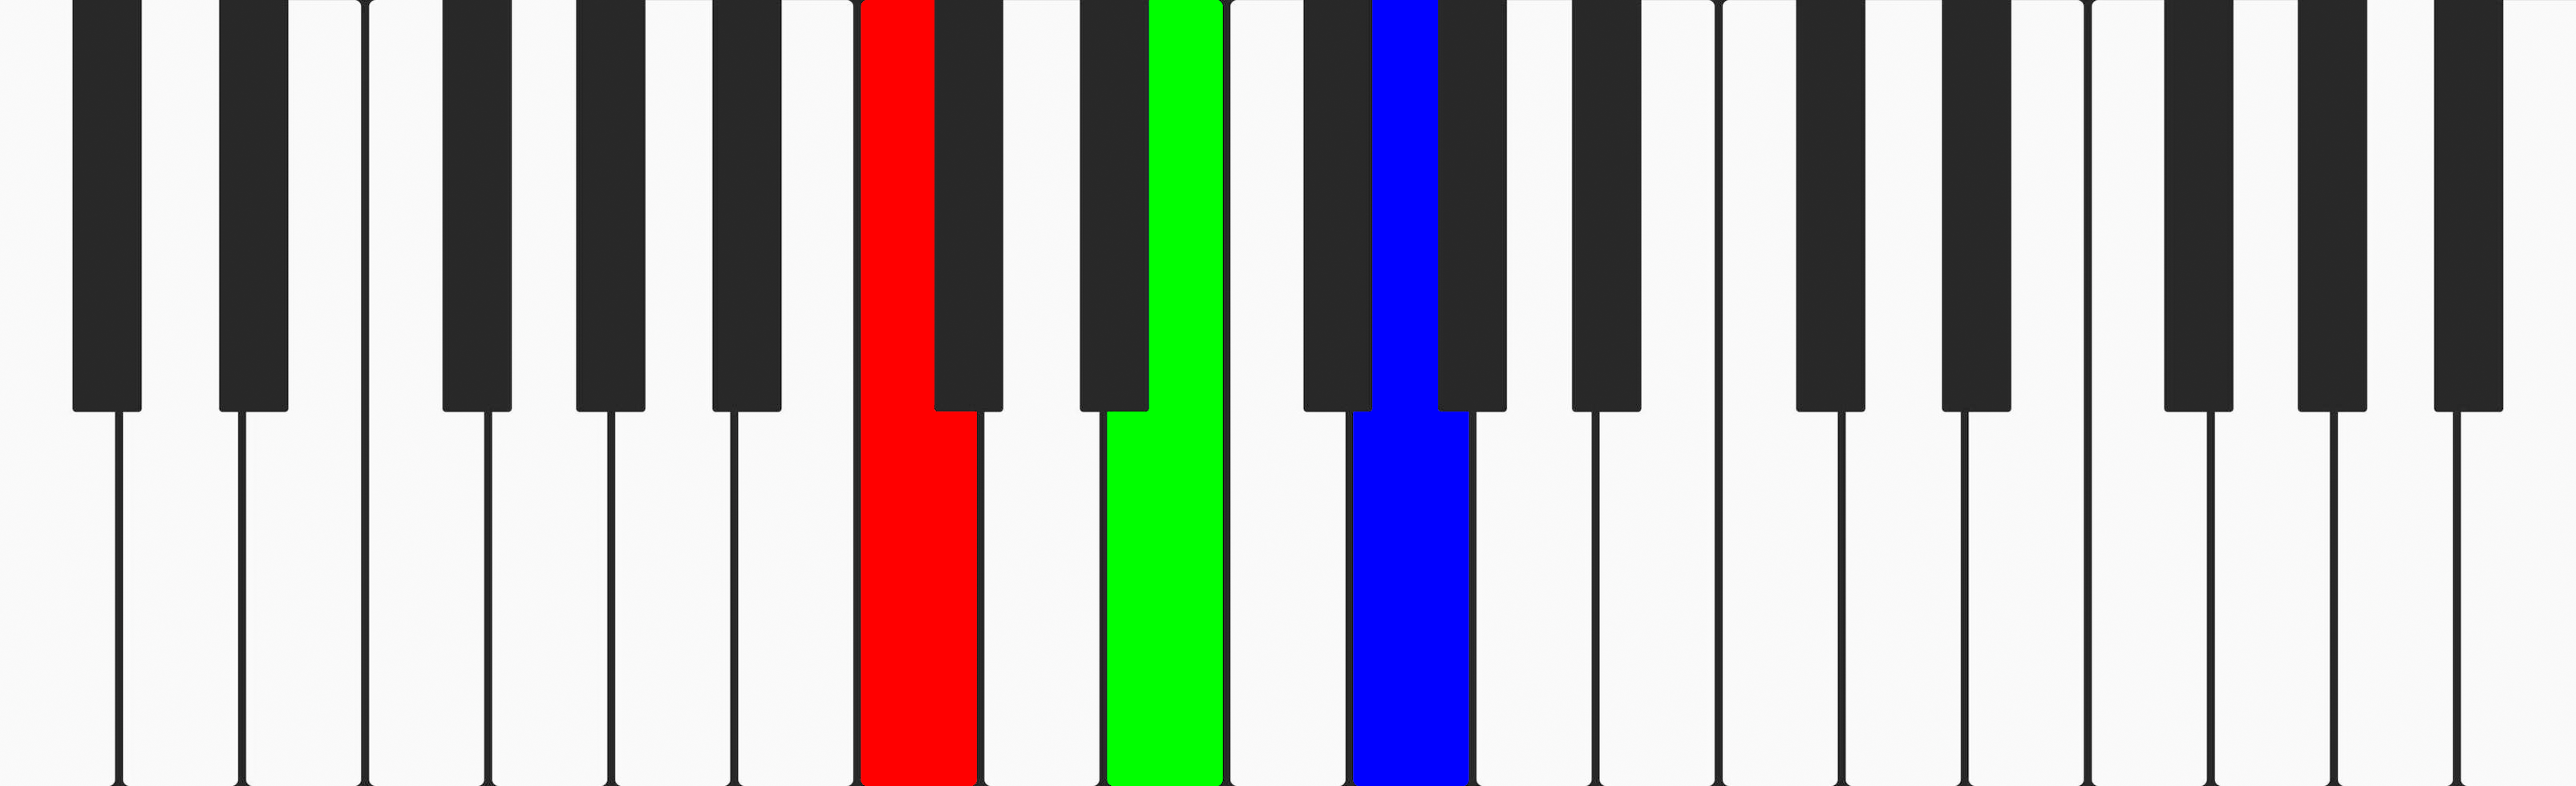
\includegraphics[width = 0.5\textwidth]{Imagenes/Bitmap/fundamental.png}
    \caption{Acorde de C en su estado Fundamental}
    \label{fig:fundamental}
\end{figure}

Una inversión consiste en la reordenación de las notas del acorde de forma que la nota mas grave no es la tónica del mismo. Por ejemplo, en una triada la nota más grave también puede ser la segunda o tercera nota del acorde, que corresponderían a la 1º y 2º inversión, como se muestra en las imágenes \ref{fig:inversion1} y \ref{fig:inversion2} respectivamente.

\begin{figure}[h]
    \centering
    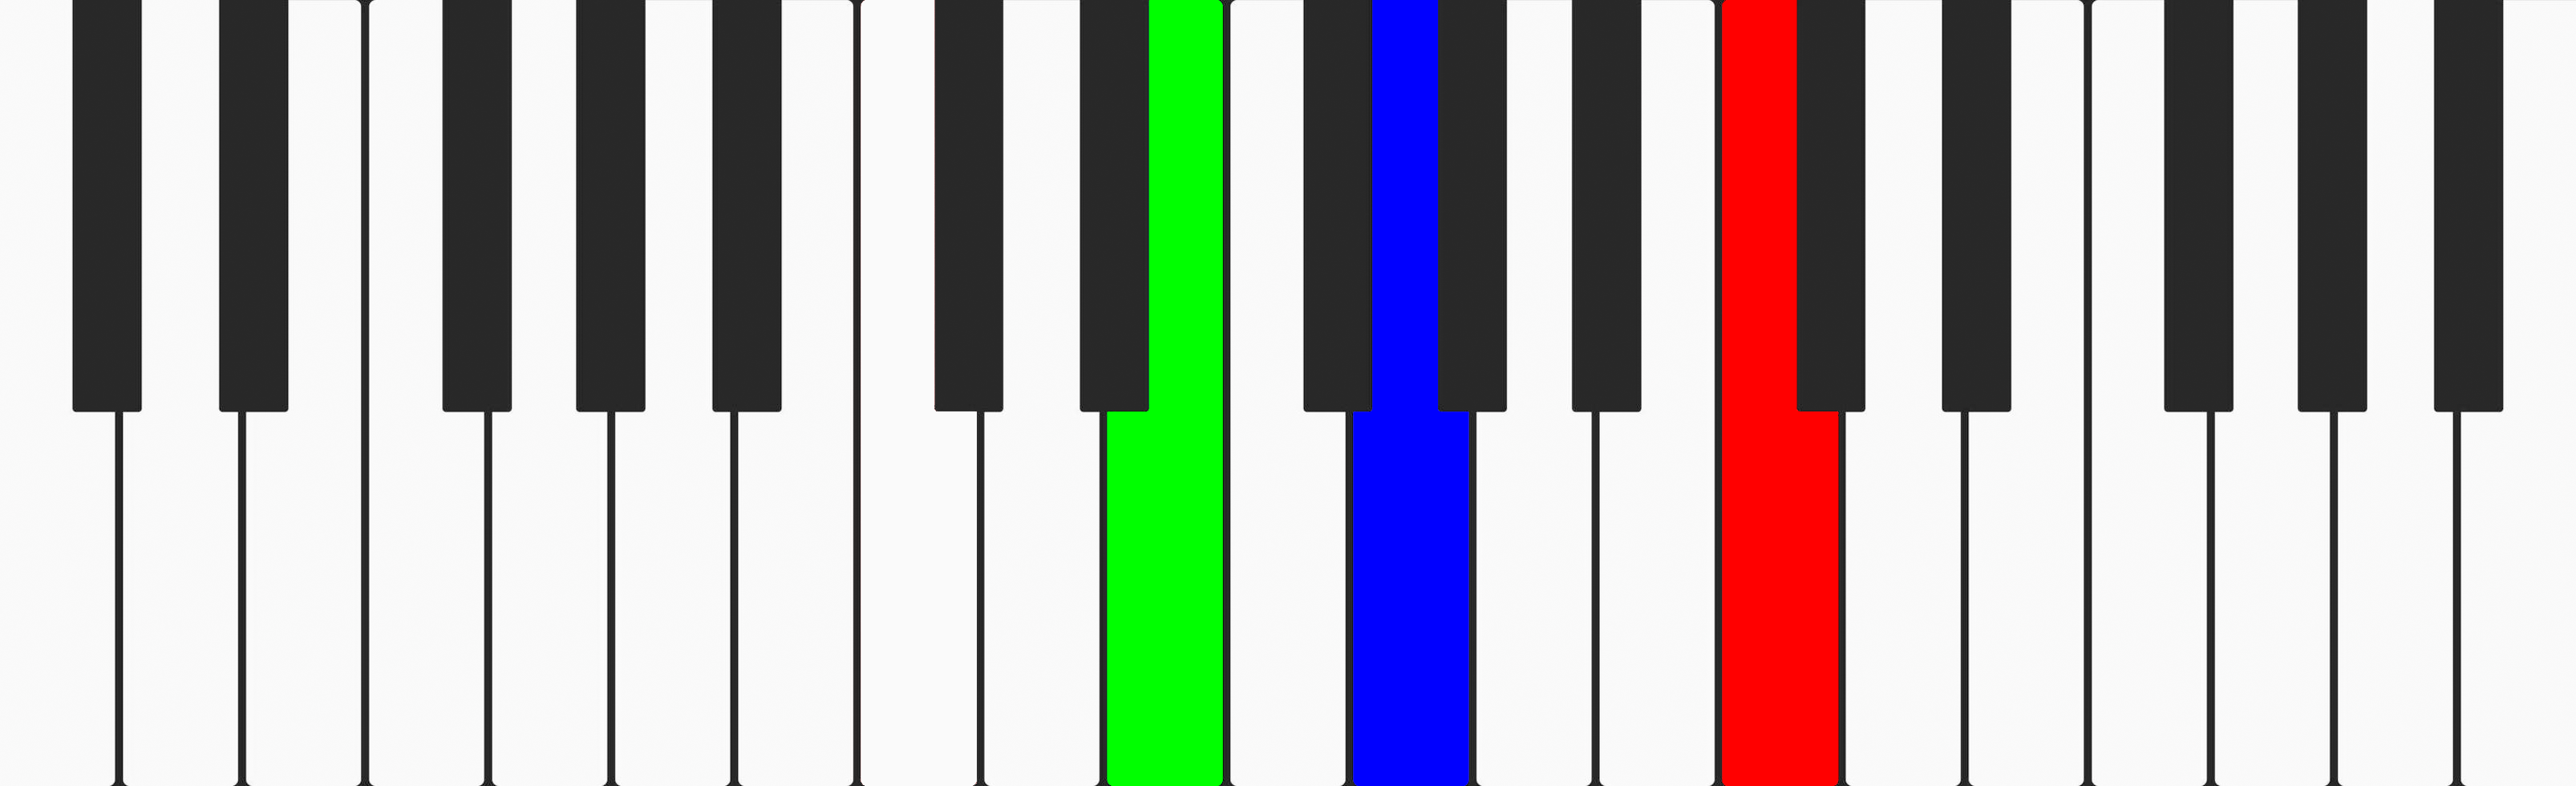
\includegraphics[width = 0.5\textwidth]{Imagenes/Bitmap/1era_inversion.png}
    \caption{Acorde de C en su 1ª Inversión}
    \label{fig:inversion1}
\end{figure}

\begin{figure}[h]
    \centering
    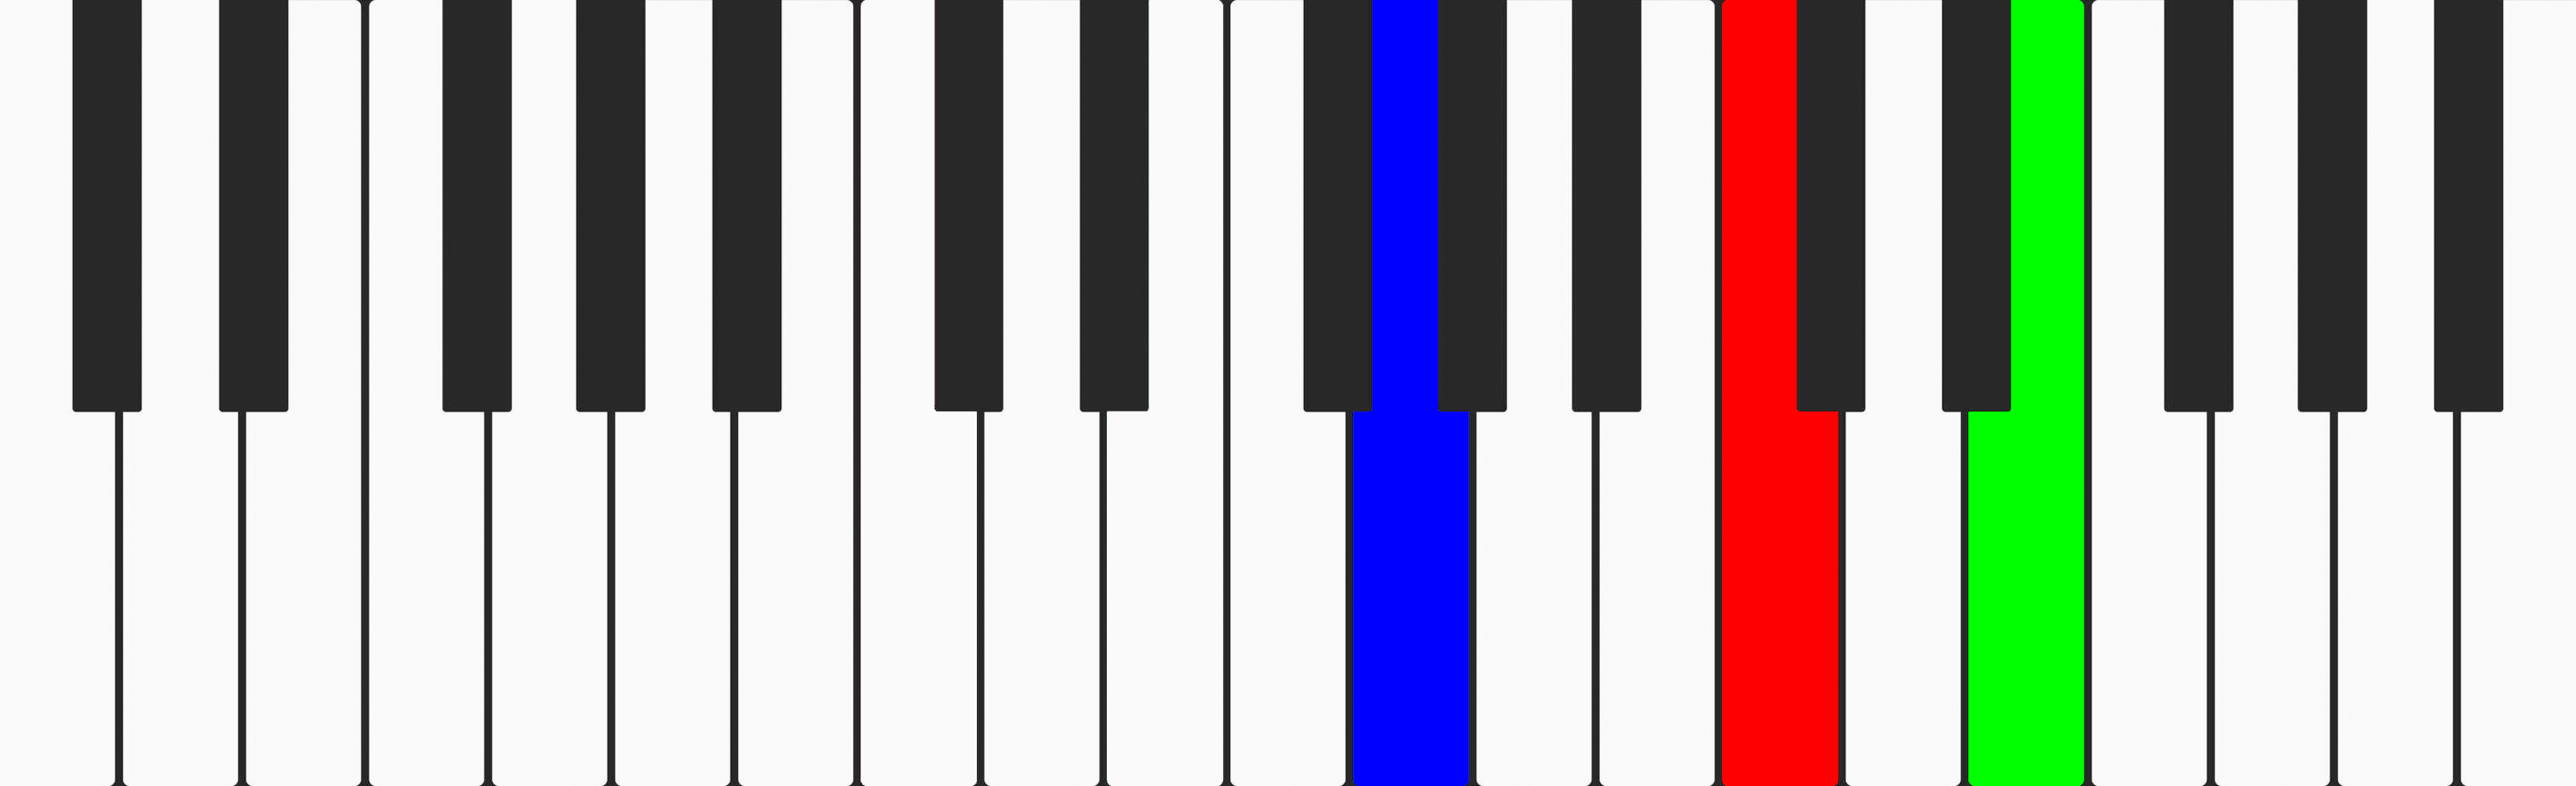
\includegraphics[width = 0.5\textwidth]{Imagenes/Bitmap/2da_inversion.png}
    \caption{Acorde de C en su 2ª Inversión}
    \label{fig:inversion2}
\end{figure}

Esta no es la única forma en la que te puedes encontrar un mismo acorde. Las notas que lo forman no tienen por qué ir consecutivas dentro de la misma octava o rango. Ejemplos en las figuras \ref{fig:inversion_extra1} y \ref{fig:inversion_extra2}. 

\begin{figure}[h]
    \centering
    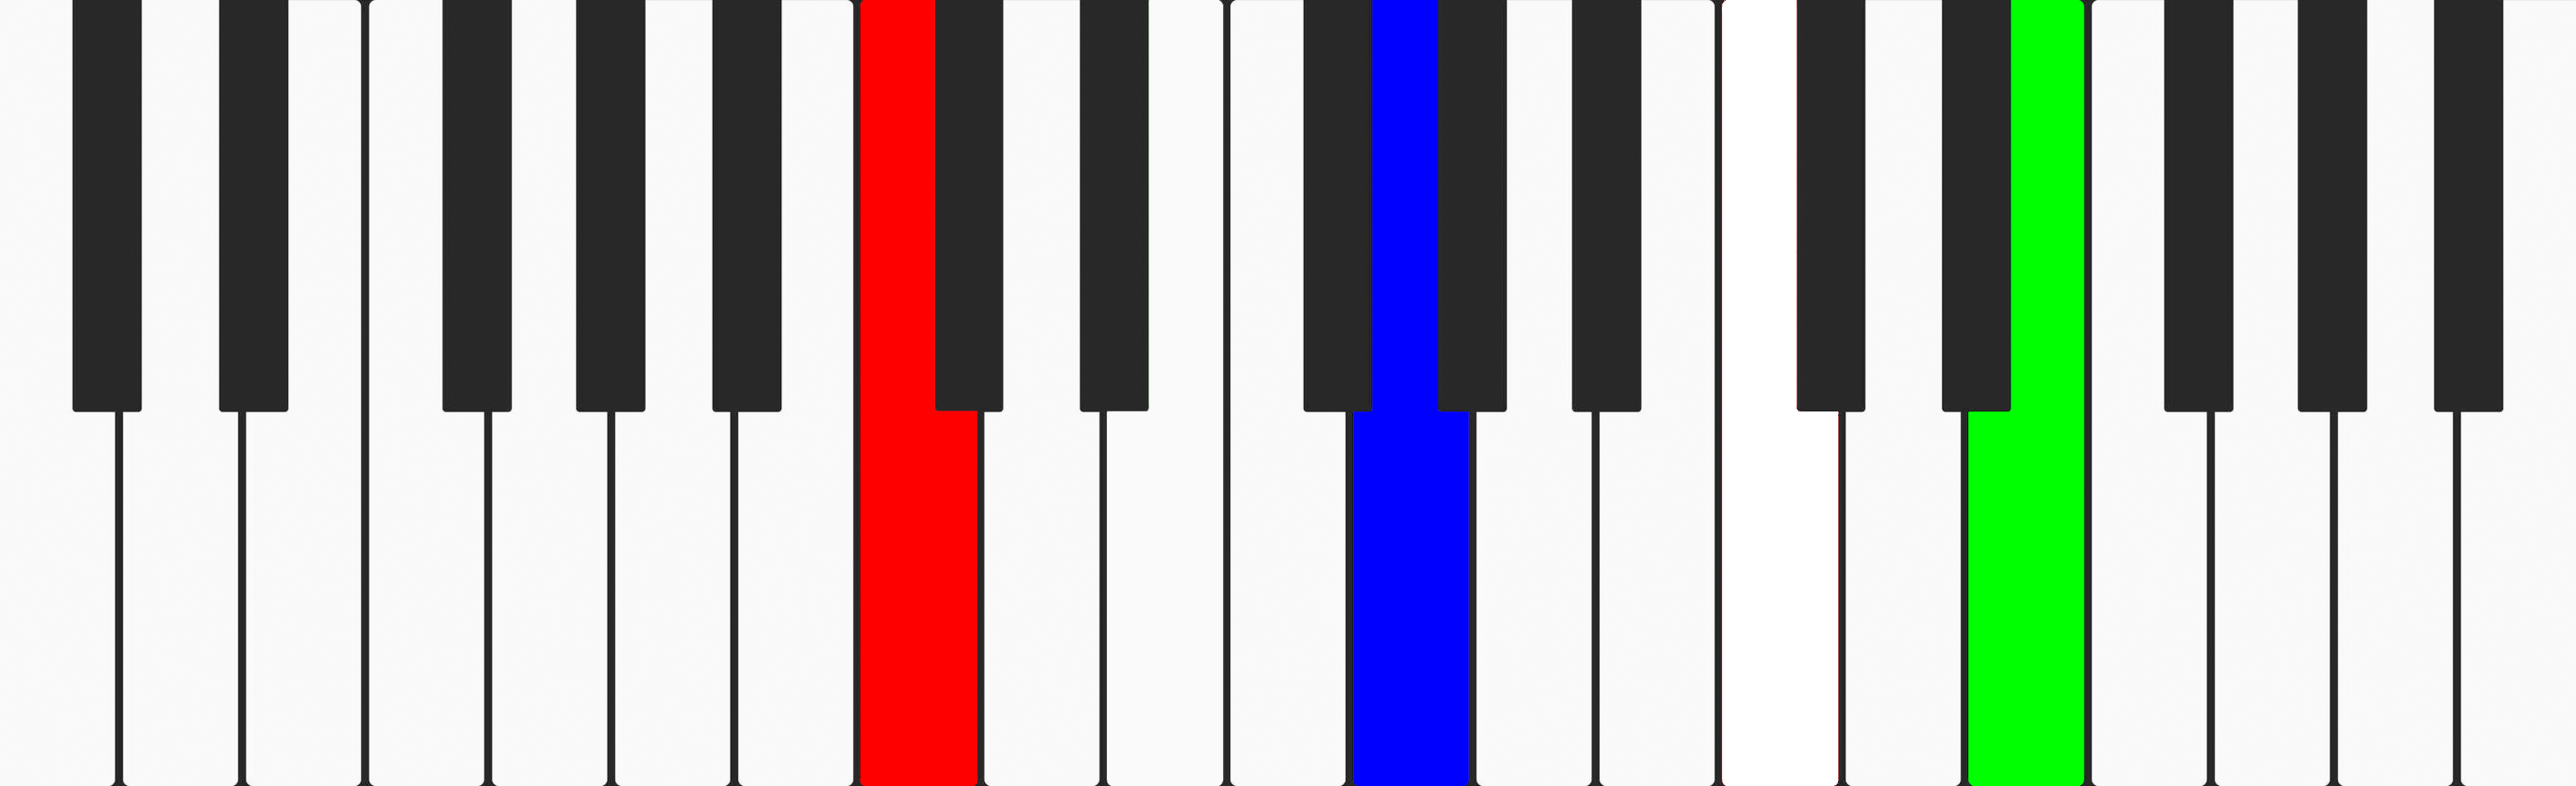
\includegraphics[width = 0.5\textwidth]{Imagenes/Bitmap/inversion_extra.png}
    \caption{Acorde de C en su estado Fundamental con sus notas en diferentes Octavas}
    \label{fig:inversion_extra1}
\end{figure}

\begin{figure}[h]
    \centering
    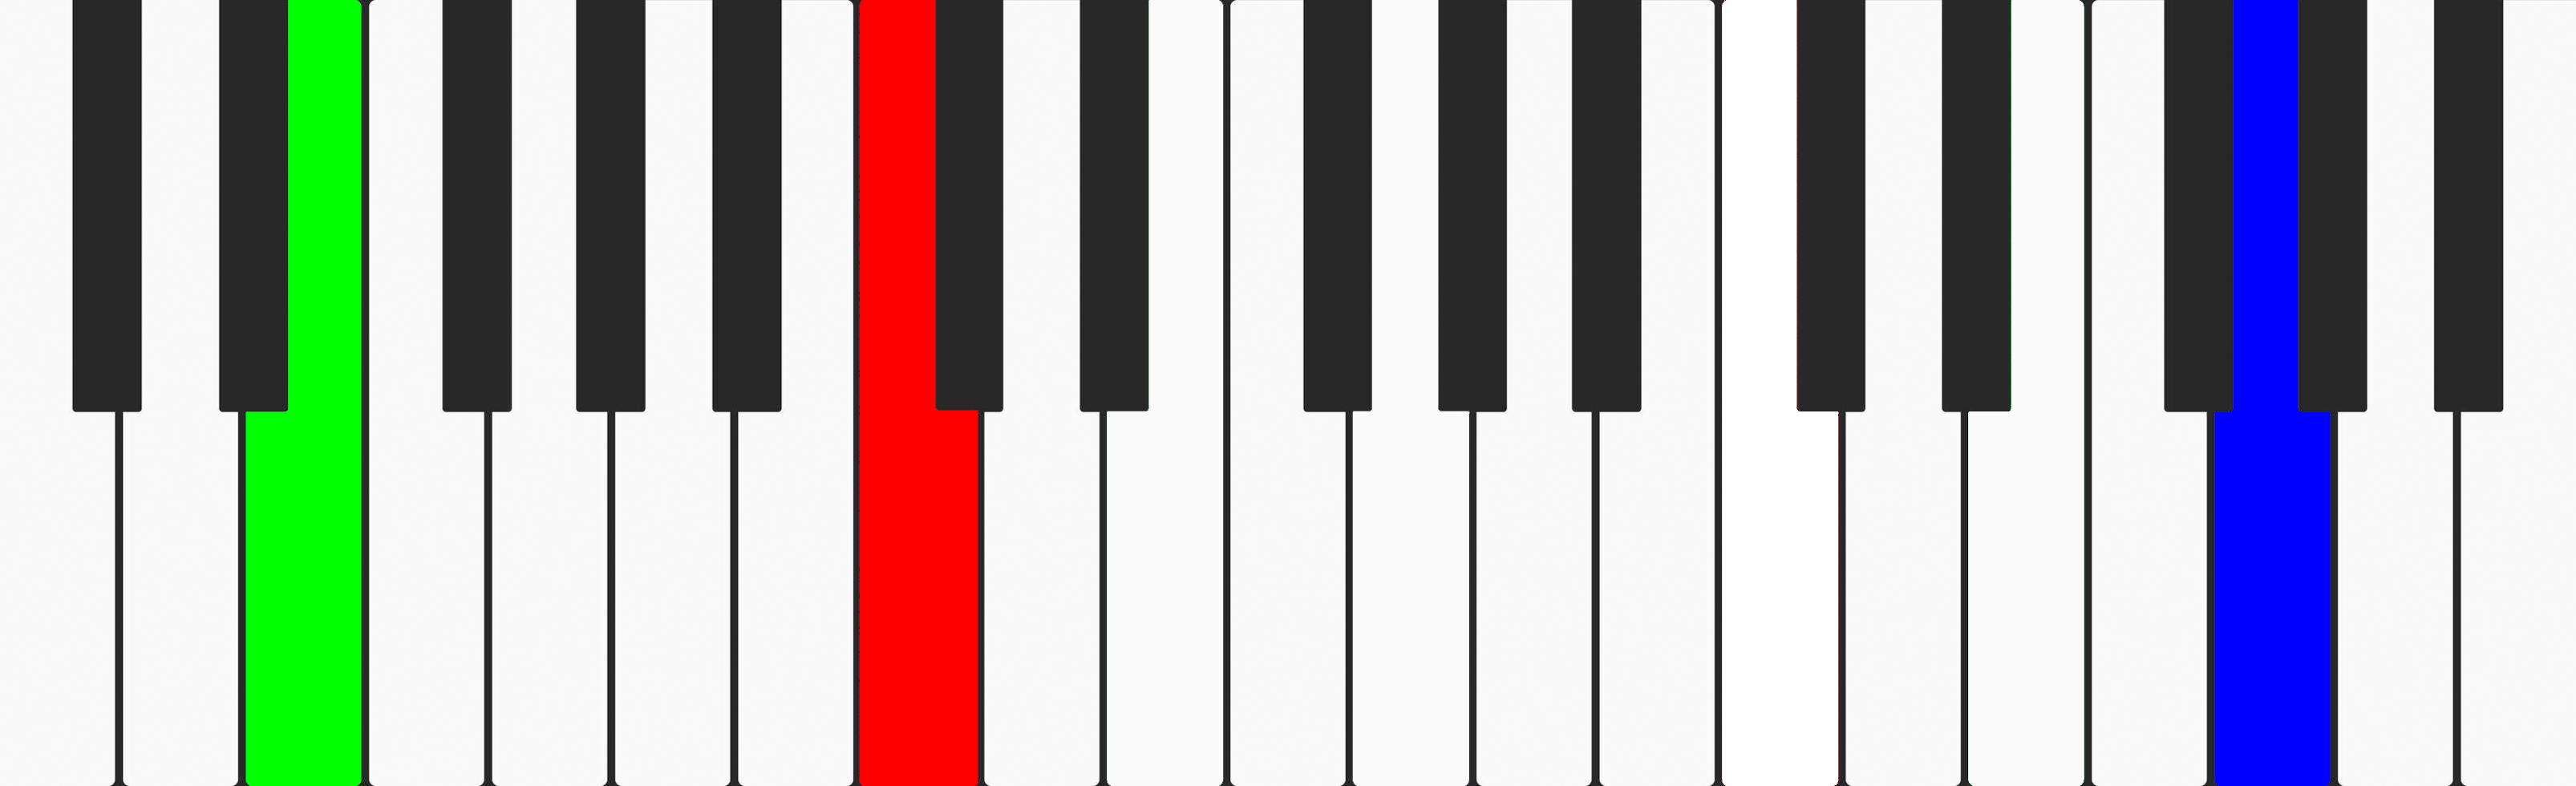
\includegraphics[width = 0.5\textwidth]{Imagenes/Bitmap/inversion_extra2.png}
    \caption{Acorde de C Invertido con sus notas en diferentes Octavas}
    \label{fig:inversion_extra2}
\end{figure}

Por supuesto, repetir notas del mismo acorde en diferentes octavas también se considera tocar dicho acorde. Ejemplo en las figura \ref{fig:inversion_extra3}.

\begin{figure}[h]
    \centering
    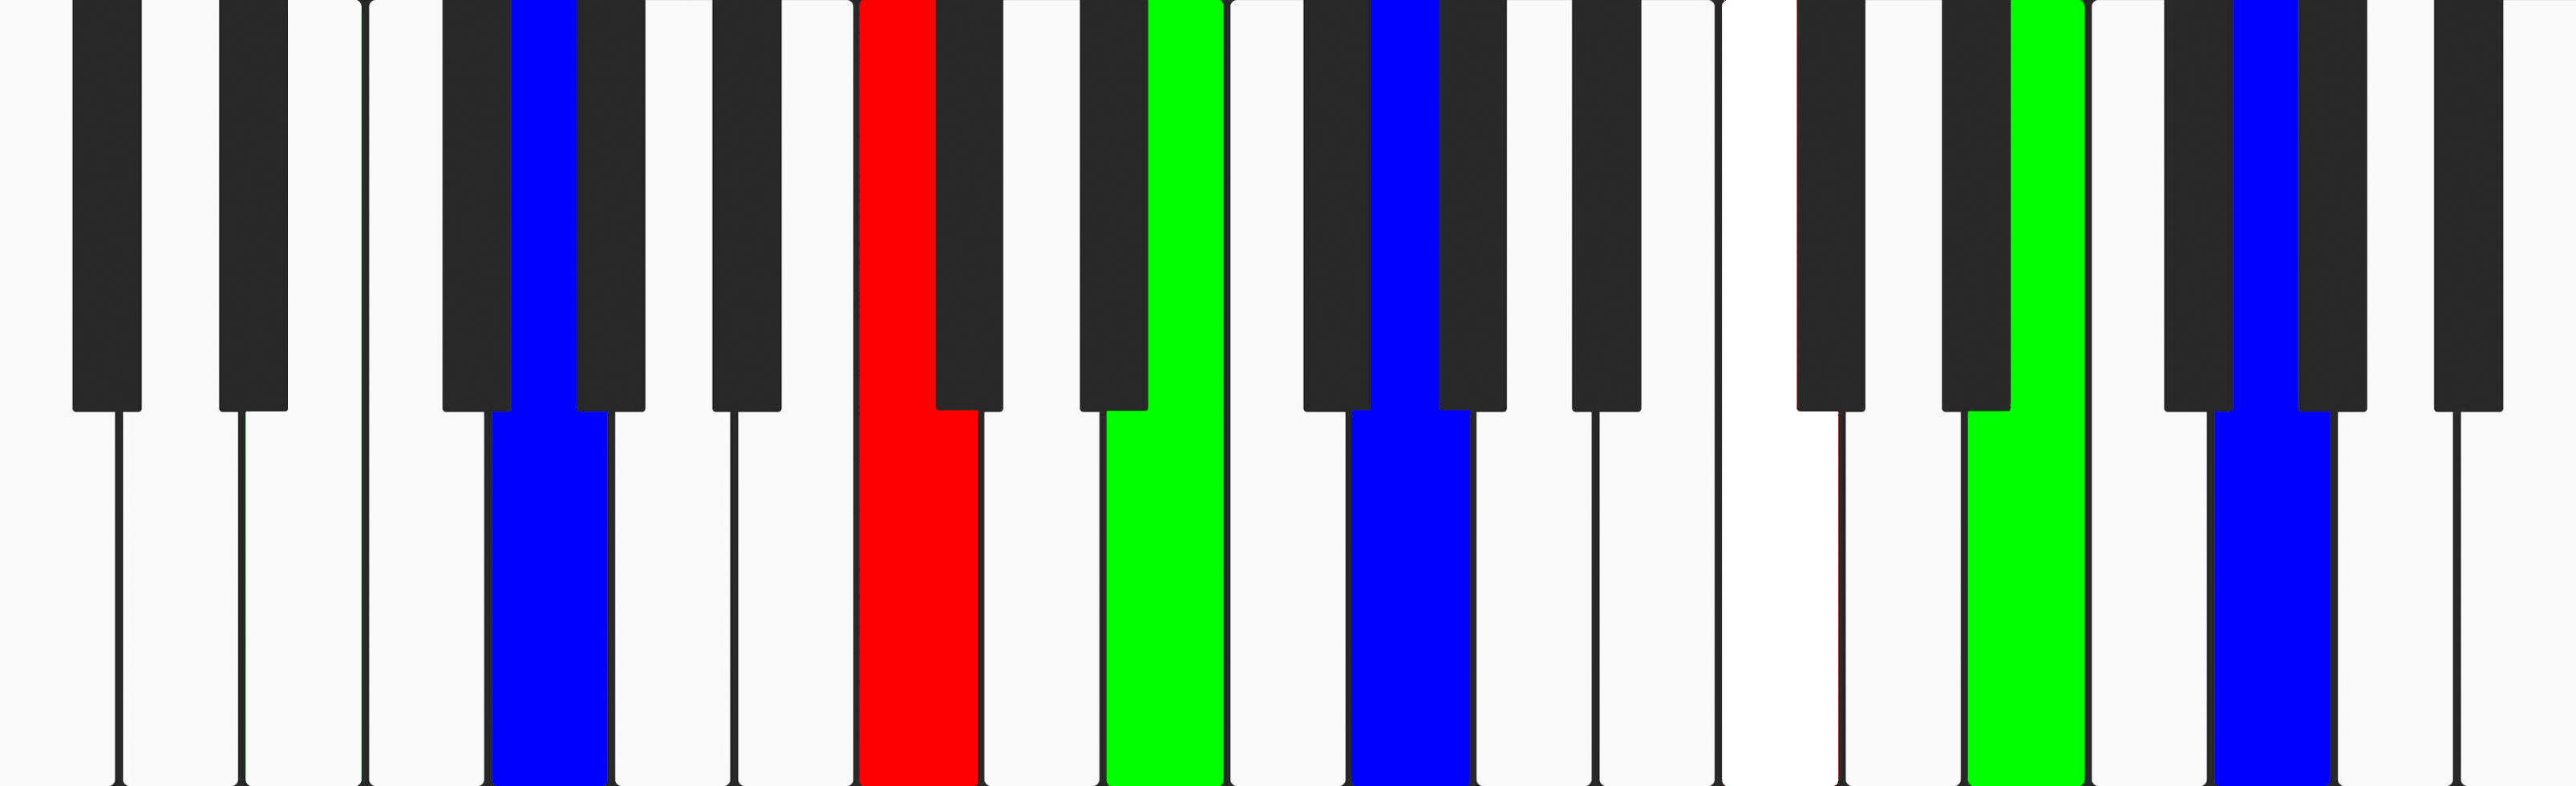
\includegraphics[width = 0.5\textwidth]{Imagenes/Bitmap/inversion_extra3.png}
    \caption{Acorde de C representado por múltiples notas}
    \label{fig:inversion_extra3}
\end{figure}

Con todos los ejemplos se quiere dejar claro que, a pesar de toda la combinatoria de respresentaciones que puede llegar a tener un mismo acorde y de las ligeras deferencias entre sus sonoridades, armónicamente simbolizan lo mismo, en este caso, el acorde de C.

\subsubsection{Arpegios}\label{subsec:arpegios}

Relacionado con las inversiones en el sentido de representar un mismo acorde pero de diferentes maneras, un apregio se define como la secuencia de la notas del acorde tocadas de manera individual y sucesiva. Este puede ser ascendente o descendente y se suele duplicar la primera nota al final.

Este y muchos otros patrones parecidos a los arpegios (y no tan parecidos también) pueden ser utilizados para tocar un mismo acorde. De nuevo, aunque las representaciones del mismo cambien, armónicamente simbolizarían lo mismo.

\subsection{Modos}

En terminos relativos, los modos de una escala son las diferenetes secuencias de intervalos que se logran al comenzar una nueva escala desde los diferentes grados de la misma. La forma más sencilla de entenderlo es con un ejemplo en términos absolutos y relativizar cada escala obtenida pasándola a intervalos como se hace en la tabla \ref{tab:modos_C} con la escala de C Mayor (C Jónico, en este contexto modal). Los modos de la escala Mayor son los más utilizados, son los  conocidos como modos griegos, cada uno conocido con un nombre propio. A pesar de ello, este mismo proceso se puede realizar con cualquier escala.

\begin{table}[h]
    \centering
    \begin{tabular}{c|c|c|c|c|c|c|c|c|c|c|c|c|c}
        \multicolumn{1}{c}{}& \textbf{C} & D & E & F & G  & A & B & \textbf{C} & D & E & F & G & A\\
        \hline
        \hline
        \textbf{Jónico} & 1 & 2 & 3 & 4 & 5 & 6 & 7  \\
        \cline{0-8}
        \textbf{Dórico} & & 1 & 2 & b3 & 4 & 5 & 6 & b7 \\
        \cline{0-0}
        \cline{3-10}
        \textbf{Frigio} &\multicolumn{2}{c|}{} & 1 & b2 & b3 & 4 & 5 & b6 & b7 \\
        \cline{0-0}
        \cline{4-11}
        \textbf{Lidio} &\multicolumn{3}{c|}{} & 1 & 2 & 3 & \#4 & 5 & 6 & 7 \\
        \cline{0-0}
        \cline{5-12}
        \textbf{Mixolidio} &\multicolumn{4}{c|}{} & 1 & 2 & 3 & 4 & 5 & 6 & b7 \\
        \cline{0-0}
        \cline{6-13}
        \textbf{Eólico} &\multicolumn{5}{c|}{} & 1 & 2 & b3 & 4 & 5 & b6 & b7 \\
        \cline{0-0}
        \cline{7-14}
        \textbf{Locrio} &\multicolumn{6}{c|}{} & 1 & b2 & b3 & 4 & b5 & b6 & \multicolumn{1}{c|}{b7} \\      
        \cline{8-14}
    \end{tabular}
    \caption{Modos Griegos}
    \label{tab:modos_C}
\end{table}

Viendo la tabla se pueden sacar varias conclusiones. La primera es que cada escala tiene tantas relativas con diferente tónica como modos tenga la propia escala. Aquí un ejemplo que sirve también para consolidar puntos descritos anteriormente: C Jónico y D Dórico son relativas entre sí porque comparten el mismo conjunto de notas, a pesar de tener distinta tónica; C Jónico y C Dórico no lo son porque aunque que comparten la misma tónica, el conjunto de notas que lo conforman es diferente, ya que el 'esqueleto' de sus escalas es diferente. La segunda conclusión es que el modo eólico es idéntico a la escala menor y que por lo tanto, en el caso del ejemplo, C Mayor (Jónico) es relativo a A menor (Eólico). Hasta ahora se ha omitido, pero toda escala Mayor tiene una relativa menor y viceversa.

A pesar de no ser tan utilizados como las escalas Mayor y menor, los modos y sobre todo, los modos griegos, son utilizados también en la música que solemos escuchar hoy por hoy. Difieren de sus relativas Mayor y menor en el centro tonal. Como la tónica es distinta, los movimientos que surgen en una composición son distintos también, lográndose así colores nuevos. Aunque los modos formen parte de un capítulo más avanzado dentro de la teoría de la armonía, el conocimiento de su existencia y su origen son cruciales para el entendimiento de varios apartados del TFG.

\section{Música generativa para videojuegos}
% Hablar de Brian Eno y la música generativa. Introducir FMOD como herramienta para música adaptativa en los videojuegos.
%Mencionar las dos posibles alternativas de generar música, es decir, de forma simbólica y luego añadir los instrumentos, o de forma directa. Decir que nos decantamos por la simbólica, pra introducir la siguiente subsección
\section{Música simbólica}
%Hablar de qué es la música simbólica, el MIDI y qué nos permite hacer.

\section{DAWs, REAPER e Instrumentos Virtuales}
% INtroducir brevemente que es una DAW, REAPER, y la necesidad de Instrumentos Virtuales para dar voz al MIDI.

%Posiblemente podams incluir aquí alguna definición más